\begin{figure*}
  \centering
  \setlength{\tabcolsep}{2.0pt}
  \begin{tabular}{cccc}
    %\toprule
    %\textbf{Fall}  & \textbf{Fall $\rightarrow$ Winter} & \textbf{Winter} & \textbf{Winter $\rightarrow$ Fall}
    %\\ \midrule
    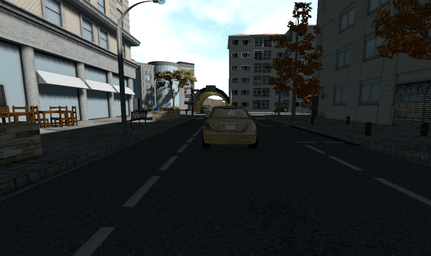
\includegraphics[width=0.24\textwidth]{figs/synthia/fall-seq1-fs8.png} &
    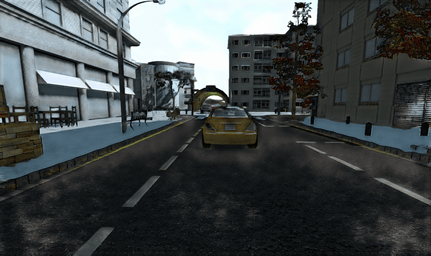
\includegraphics[width=0.24\textwidth]{figs/synthia/fake-winter-seq1-fs8.png} &
    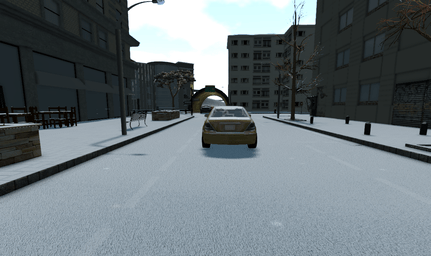
\includegraphics[width=0.24\textwidth]{figs/synthia/winter-seq1-fs8.png} &
    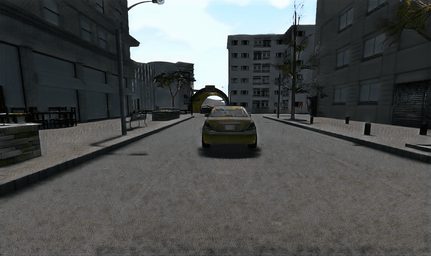
\includegraphics[width=0.24\textwidth]{figs/synthia/fake-fall-seq1-fs8.png}
    \\
	   (a) Fall & (b) Fall $\rightarrow$ Winter & (c) Winter & (d) Winter $\rightarrow$ Fall
    %\includegraphics[width=0.24\textwidth]{figs/synthia/fall-seq2-fs8.png} &
    %\includegraphics[width=0.24\textwidth]{figs/synthia/fake-winter-seq2-fs8.png} &
    %\includegraphics[width=0.24\textwidth]{figs/synthia/winter-seq2-fs8.png} &
    %\includegraphics[width=0.24\textwidth]{figs/synthia/fake-fall-seq2-fs8.png}
    %\\
    %\includegraphics[width=0.24\textwidth]{figs/synthia/fall-seq4-fs8.png} &
    %\includegraphics[width=0.24\textwidth]{figs/synthia/fake-winter-seq4-fs8.png} &
    %\includegraphics[width=0.24\textwidth]{figs/synthia/winter-seq4-fs8.png} &
    %\includegraphics[width=0.24\textwidth]{figs/synthia/fake-fall-seq4-fs8.png}
    %\\
    %\includegraphics[width=0.24\textwidth]{figs/synthia/fall-seq5-fs8.png} &
    %\includegraphics[width=0.24\textwidth]{figs/synthia/fake-winter-seq5-fs8.png} &
    %\includegraphics[width=0.24\textwidth]{figs/synthia/winter-seq5-fs8.png} &
    %\includegraphics[width=0.24\textwidth]{figs/synthia/fake-fall-seq5-fs8.png}
    %\\
    %\bottomrule
  \end{tabular}
  \caption{
    \textbf{Cross Season Image Translation.} Example image-space conversions for the SYNTHIA seasons adaptation setting.
    We show real samples from each domain (Fall and Winter) alongside conversions to the opposite domain.
    }
  \label{fig:synthia}
\end{figure*}
